We have developed a server of the detection/prediction stage of the  AAnchor algorithm at \url{http://bioinfo3d.cs.tau.ac.il/AAnchor/}.
The server outputs the detection results in PDB format, so that they could be displayed in commonly used programs such as UCSF Chimera \cite{Pettersen2004UCSFAnalysis}.
Figure ~\ref{f:t2} illustrates the server output as shown in UCSF Chimera.
Yellow spheres, which mark the predicted locations of prolines, are superimposed with 
the reference atomic model. 
\begin{figure}
  \caption{Detection of proline residues in a $ 2.9 \; \AA$ Cryo EM map. Yellow spheres show the predicted centers of mass for each of the detected amino acids. } \label{f:t2}
  \centering
    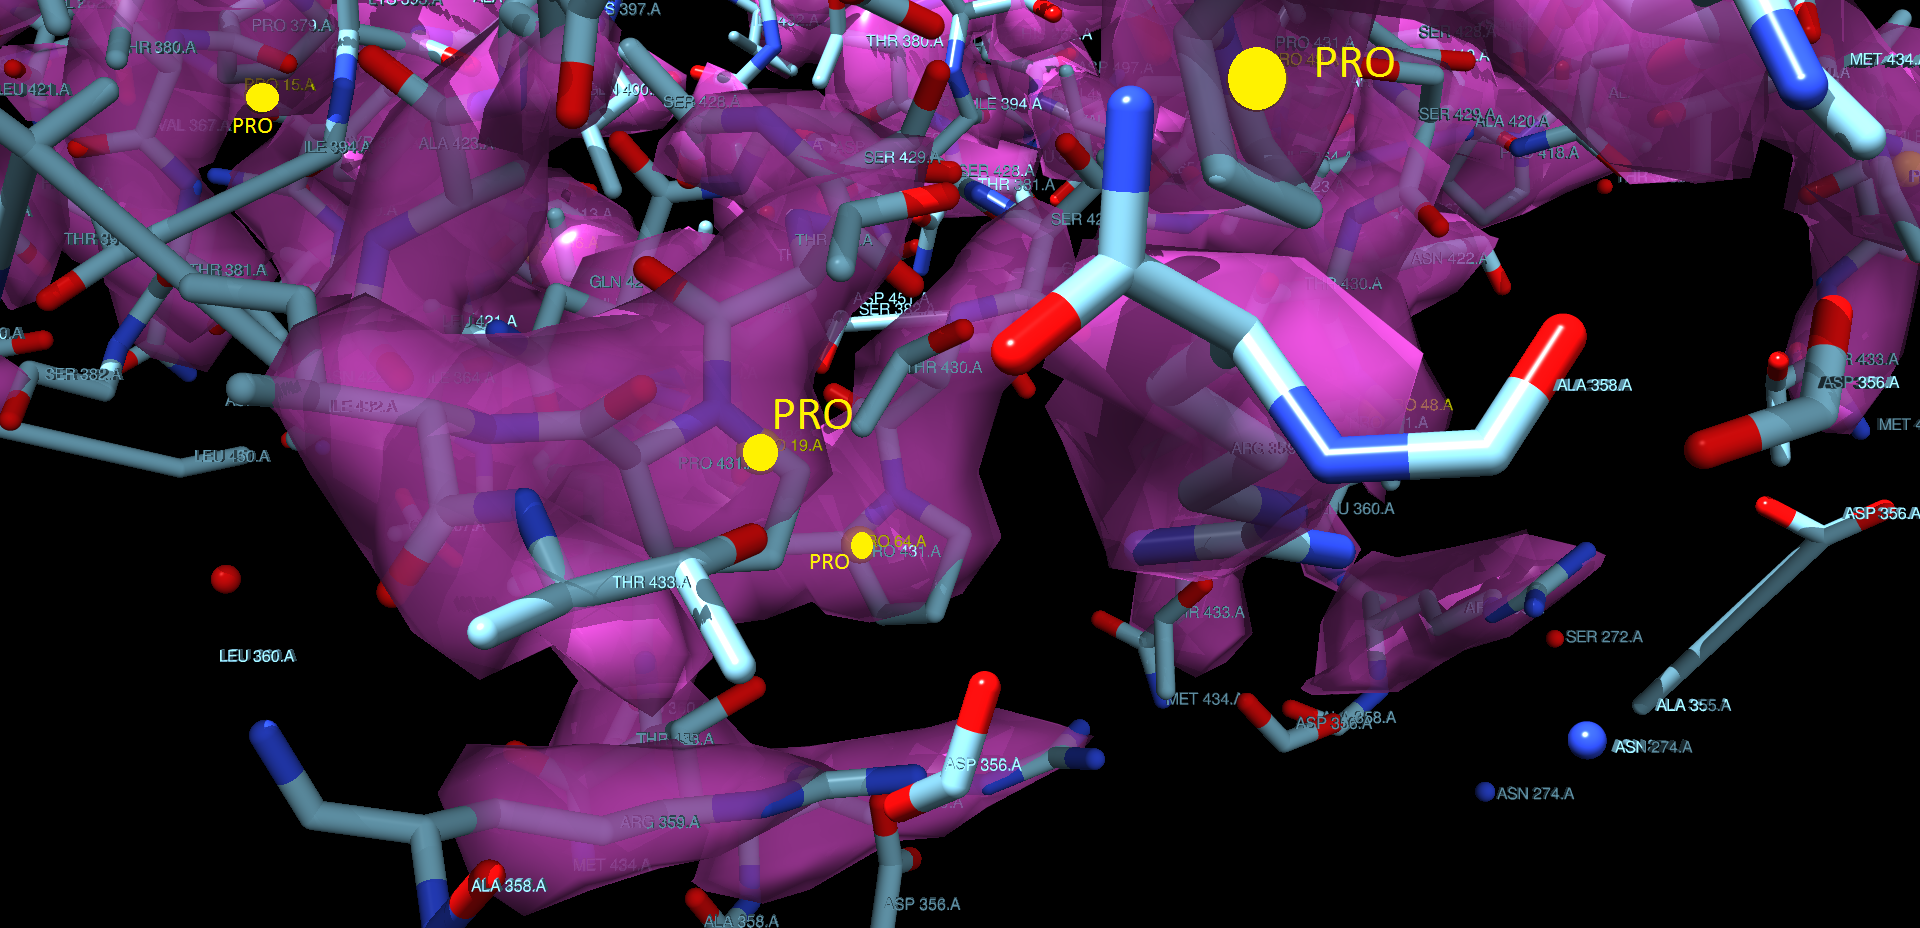
\includegraphics[width=0.5\textwidth]{pics/t2.png}
\end{figure}
